\DiaryEntry{Groups, II}{2016-03-03}{Algebra}

In this post, we consider the operation and symmetries of an equilateral
triangle.

\subsubsection{Identity}\label{identity}

The identity transformation leaves the triangle as it is.

\begin{figure}
\centering
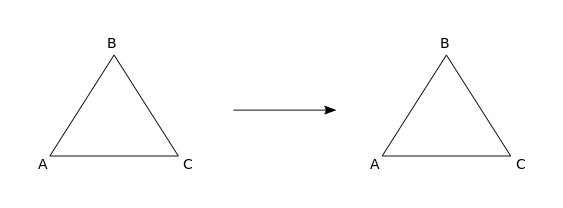
\includegraphics[scale=0.7]{images/groups_02_1.png}
\caption{Page1}
\end{figure}

We can write the effect of the transformation as a permutation matrix of
the points A, B, and C.

\[
e=\begin{pmatrix}
A & B & C\\
A & B & C\end{pmatrix}
\]

\subsubsection{Rotation}\label{rotation}

There are two rotations, clockwise and counter-clockwise possible.

\begin{figure}
\centering
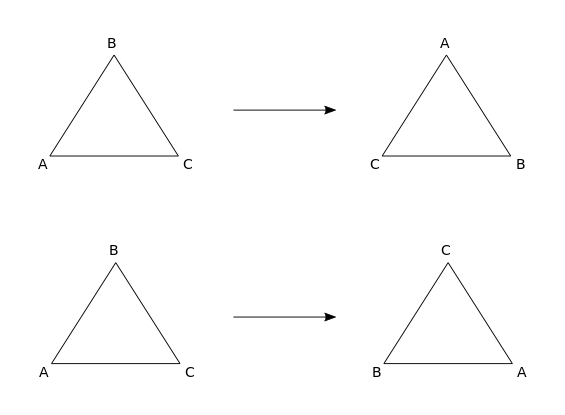
\includegraphics[scale=0.7]{images/groups_02_2.png}
\caption{Page1}
\end{figure}

The clockwise rotation (upper one) has the following permutation matrix:

\[
\rho_1=\begin{pmatrix}
A & B & C\\
B & C & A\end{pmatrix}
\]

Because of the rotation, the point A becomes the point B and so on.

The counter-clockwise rotation (lower one) has the following permutation
matrix:

\[
\rho_2=\begin{pmatrix}
A & B & C\\
C & A & B\end{pmatrix}
\]

\subsubsection{Reflection}\label{reflection}

There ae three reflections possible; each leaving one triangle point the
same.

\begin{figure}
\centering
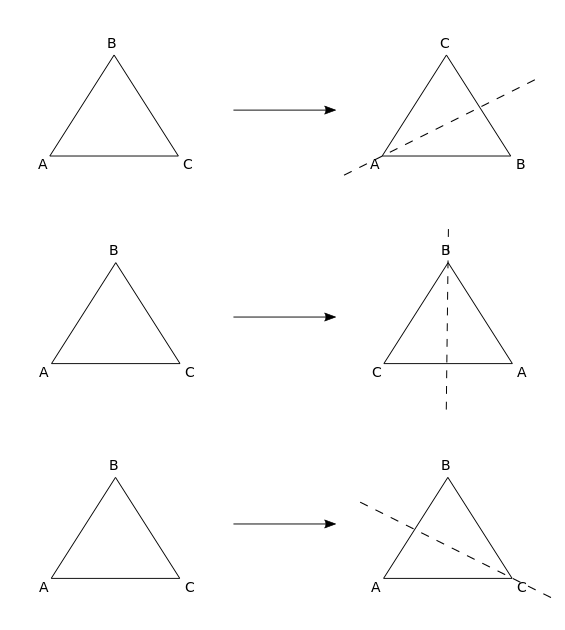
\includegraphics[scale=0.7]{images/groups_02_3.png}
\caption{Page1}
\end{figure}

The first reflection has the following permutation matrix

\[
\mu_1=\begin{pmatrix}
A & B & C\\
A & C & B\end{pmatrix}
\]

The second reflection has the following permutation matrix

\[
\mu_2=\begin{pmatrix}
A & B & C\\
C & B & A\end{pmatrix}
\]

The third reflection has the following permutation matrix

\[
\mu_3=\begin{pmatrix}
A & B & C\\
B & A & C\end{pmatrix}
\]

\subsection{Group Interpretation}\label{group-interpretation}

In total, there are 6 operations for the triangle: 1 ``do-nothing''
identity, 2 rotations, and 3 reflections. These 6 operations form a
group with the function \(\star\) being the combination of two such
permutations: the function is associative, there exists an identity
element (the first ``identity'' permutation above), and there exists an
inverse element (a permutation is a one-to-one mapping; therefore it has
an inverse).

As an example of combination, consider the effect of the subsequent
execution of \(\mu_1\) and \(\rho_1\) on the point A:
\((\mu_1 \rho_1)(A) = \mu_1(\rho_1(A)) = \mu_1(B) = C\). The same for
points B and C yields \((\mu_1 \rho_1)(B) = B\) and
\((\mu_1 \rho_1)(C) = A\). We can again write this as a permutation
matrix

\[
\mu_1 \rho_1 = \begin{pmatrix}
A & B & C\\
C & B & A\end{pmatrix}
\]

and from this we see that the combined effect of the two permutations
equals \(\mu_2\).

\subsubsection{Multiplication Table}\label{multiplication-table}

We can capture the combined effect of two operations / permutations by
means of a multiplication table (the table is to be read ``row-first''):

\[
\begin{array}{c|cccccc}
\star  & e     & \rho_1 & \rho_2 & \mu_1 & \mu_2 & \mu_3 \\
\hline
e     & e     & \rho_1 & \rho_2 & \mu_1 & \mu_2 & \mu_3 \\
\rho_1 & \rho_1 & \rho_2 & e     & \mu_3 & \mu_1 & \mu_2 \\
\rho_2 & \rho_2 & e     & \rho_1 & \mu_2 & \mu_3 & \mu_1 \\
\mu_1  & \mu_1  & \mu_2  & \mu_3  & e    & \rho_1& \rho_2\\
\mu_2  & \mu_2  & \mu_3  & \mu_1  & \rho_2 & e    & \rho_1\\
\mu_3  & \mu_3  & \mu_1  & \mu_2  & \rho_1 & \rho_2& e
\end{array}
\]

We see the combination of \(\mu_1\) and \(\rho_1\) in the row \(\mu_1\)
and column \(\rho_1\) being \(\mu_2\).

From the table we also observe that the group is \textbf{not} abelian as
the oeration is \textbf{not} commutative; e.g.
\(\rho_1 \star \mu_1 \neq \mu_1 \star \rho_1\).

\subsubsection{Other Interpretation /
Subgroups}\label{other-interpretation-subgroups}

A slightly different interpretation is to define a ``start''
configuration e of a triangle and to consider the effects one
transformation has on this start configuration. If we define the start
configuration as the first triangle above, then \(\rho_1\) defines a
clockwise rotation of this triangle. Subsequent transformations can be
grouped into one compound transformation as by the multiplication table
above.

This interpretation allows to investigate the subgroups of the group. We
start with e and repeatedly apply \(\rho_1\), in order to receive the
following sequence: e
\(\rightarrow \rho_1 \rightarrow \rho_2 \rightarrow\) e. In a similar
spirit we obtain e \(\rightarrow \mu_1 \rightarrow\) e, e
\(\rightarrow \mu_2 \rightarrow\) e, and e
\(\rightarrow \mu_3 \rightarrow\) e.

Each of these subgroups is cyclic; however, no single element generates
the whole group, therefore the whole group is not cyclic. The Figure
below shows these cyclic subgroups.

\begin{figure}
\centering
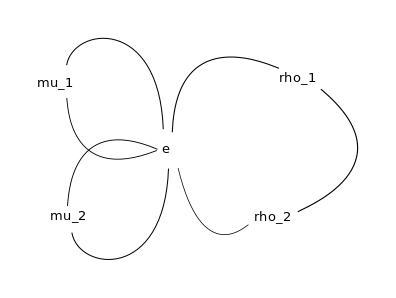
\includegraphics[scale=0.7]{images/groups_02_4.png}
\caption{Page1}
\end{figure}

\subsubsection{Relation to Permutation
Groups}\label{relation-to-permutation-groups}

In this special case of triangles, the 6 operations represent all
permutations of the three triangle points A, B, C. Therefore, the group
we described above is actually the permutation group \(S_3\).

Permutations are covered in a later post (Groups, IV).

